\chapter{An Autonomous Robotic Team for the Rapid Characterization of Novel Environments}

\section{Rapid Georectification and Processing of Pushbroom Hyperspectral Imagery}

Recent developments in hyperspectral imaging technology have led to dramatic reductions in both size and weight of imaging platforms. Due to these improvements, it is now possible to incorporate the technology as the payload of highly mobile autonomous aerial vehicles such as drones. However, the massive volume of hyperperspectral datacubes poses significant computational challenges to their adoption in real-time applications. In this paper, we demonstrate a procedure for the rapid georeferencing of pushbroom imagery and demonstrate its application for real-time remote sensing... Results indicate that a typical image can be processed in ~10 seconds while it takes $x$ seconds to capture. 



For decades, multi-spectral imagers* have seen wide spread adoption in the remote sensing community as a means to take advantage of the wealth of information contained in the reflectance spectra of materials. In addition to the three color filters of traditional cameras, *multi-spectral* imagers, like those deployed on MODIS, Sentinel 2, and other satellite missions, capture many additional features by utilizing wavelength bands ranging from the near-UV, through the visible spectrum, and into the Infrared. With this additional information, multi-spectral remote sensing platforms are able to aid in a variety of domains from tracking land change, characterizing deforestation, monitoring erosion, evaluating crop health, and many others (add references here). 

(**add a figure showing the different wavelength bands of publically available satellites**)

These uses are justified by the reflectance features of materials across the electromagnetic spectrum; water has vibrational modes in the IR, pigments have absorption peaks in the visible, etc...(discuss the particular features present in different regions of the reflectance spectrum). Many currently used spectral indices like the *normalized difference vegatation index* (NDVI) take advantage of these spectral regions by comparing ratios of pigment sensitive passbands to the constant signals infrared to infer the abundance of chlorophyll, and consequently, the health of plants, to identify forest canopy, etc..(**add citations and expand**)

However, despite the plethora of successful applications of multi-spectral imaging, more can be accomplished with the additional information provided by fully resolved spectra. For example, in the laboratory, spectrophotometry allows the direct determination of the concentrations of chemicals constituents in solution (**add more detail and references**) by deconvolution of a sample spetrum against libraries carefully collected of reference spectra: individual chemicals be uniquely identified by the characterstic location and shape of their absorption features. We should mention something about algal blooms-- harmful species display shifted reflectance peaks that can be used to identify toxic species. This information is effectively filtered away by the broad passbands of existing (find the spectra used in that book that show the different species of algae). To that end, *hyperspectral imagers* (HSI), which sample hundreds of wavelength binds at each pixel, have become the natural next step for remote sensing platforms with many planned to deployed in the coming years (**add references about soon-to-be-deployed HSI satellites**). 


At the terrestrial level, drones (commonly, quadcoptrs, octocopters, and other similar multi-rotor craft) equipped with cameras are able to utlize techniques of photogrametry together with continuously sampled imagery to produce high quality digital elevation maps, high quality mosaics, 3-dimensional reconstructions, etc... These capabilities provide significant aid for structural analysis, smart agriculture, etc... Today, kilogram-scale HSI can be comfortably mounted to the payload of film-scale drones such as the AltaX and advancements in spectral sensing such as (**reference Ethan Minot's recent paper**) suggest that sizes of HSI will continue to shrink further expanding their application in this domain. 

The increased spectral resolution of HSI systems poses unique challenges to their adoption for real time applications primarily stemming from the considerable size of generated data files. Current data collection workflows see researchers first perform the aerial survey (data collection) and then transfer data to ground based computers for post processing. This workflow is well established in the remote sensing community where, as an example, compressed raw imagery from Sentinel-2 are transferred to the ground and then subsequently post processed into their final L1C (top of atmosphere) and L2A (bottom of atmosphere) data products ((**add citation here**)). Drone based applications often operate in a similar manner: images or video are collected by a survey and then post-processed and analyzed with software such as Open Drone Map to produce the desired data products (tile mosaics, 3d reconstructions, etc.) (**add citation**). For an HSI platform to function in real time, three key computational tasks are critical: 
1. **FileIO**: captured imagery need to be quickly read by the on-board processing computer
2. **Post-processing**: Raw imagery need to be rapidly converted to the chosen data product (typically, Reflectance), and importantly, must be georeferenced so that each image pixel can be located on the ground.
3. **Ground Transfer**: Sufficient wireless communication must be avaiable to transmit the final 

The first can be readily accomplished by means of light weight, high volume solid state drives. To address the second, we need both sufficient compute and optimized processing software. Finally, ground transfer of final post-processed data products can be accomplished in a variety of ways. As we rarely need the full hyper-spectral datacube right away, once can generate the desired data products on board (NDVI for example) and transfer only the relevant information to a ground station 

We should now make the argument about the need for improved methods for processing of HSI due the their dramatically larger size, i.e. the standard workflow of collecting imagery and then post processing (re: Open Drone Map) is a fantastic and well tested solution but prevents the use in time-critical applications. We can also reference the continued improvements to single-board computers such as the raspberry pi 4b (8 Gb of Ram), Jetson family (GPU equipped), and intel nuc (powerful work horses with miniscule form factors). To make real-time possible we need two things: 
1. Conversion from raw data (digital counts) to physical units like Reflectance 
2. Georeferencing of captured imagery so features can be quickly geolocated

We can always re-process the imagery later for an in-depth reanalysis, but for time-critical applications, we need all of the processing to happen on board the drone. 


Add a paragraph about georeferencing in particular:
- Georectification = georeference + orthorectification
- outline other papers that have discussed georectification techniques:
    - ground control points  (not reasonable for dangerous or water-based environments)
    - IMU / GPS
    - different type of sensors: square, pushbroom, whiskbroom

Discuss configurations of imagers and the development of georeferencing strategies, e.g. starting with the Muller paper and going to today. Mention potential for the incorporation of digital elevation maps together enabled by GPUs and video game engines (**reference that one paper that suggests using Unity or something similar for the projective geometry optimized for Cuda on NVIDIA GPUs**).

In our previous work, we demonstrated a prototype autonomous robot team employing a drone based hyper-spectral imager which can learn the mapping from reflectance spectra to concentrations of variety of chemicals-of-concern by utilizing the information contained in the reflectance spectra captured with a HSI together with a  \cite{robot-team-1}. In this paper, we present a procedure based on the method of \cite{muller-georeferencing} for the rapid processing and georeferencing of imagery captured by a pushbroom HSI mounted on an autonomous. Associated code can be freely accessed and downloaded in (**add reference to our repository**)

(**This point can be saved for the supervised learning paper**) what we really want (usually) isn't the full spectra at each pixel 

IMU - inertial measurement unit


\subsection{Autonomous Aerial Vehicle}

subsection detailing the robot team, and specifically, the drone setup (HSI, NUC, Flir, etc...) 
- HSI takes images 
- IMU/GPS onboard position/orientation determination
- Intel NUC 1: manages HSI
- SSD
- Intel NUC 2: Processing 
- Ubiquity long-range wifi antenna (for streaming data products)

\begin{figure}[h]
    \centering
    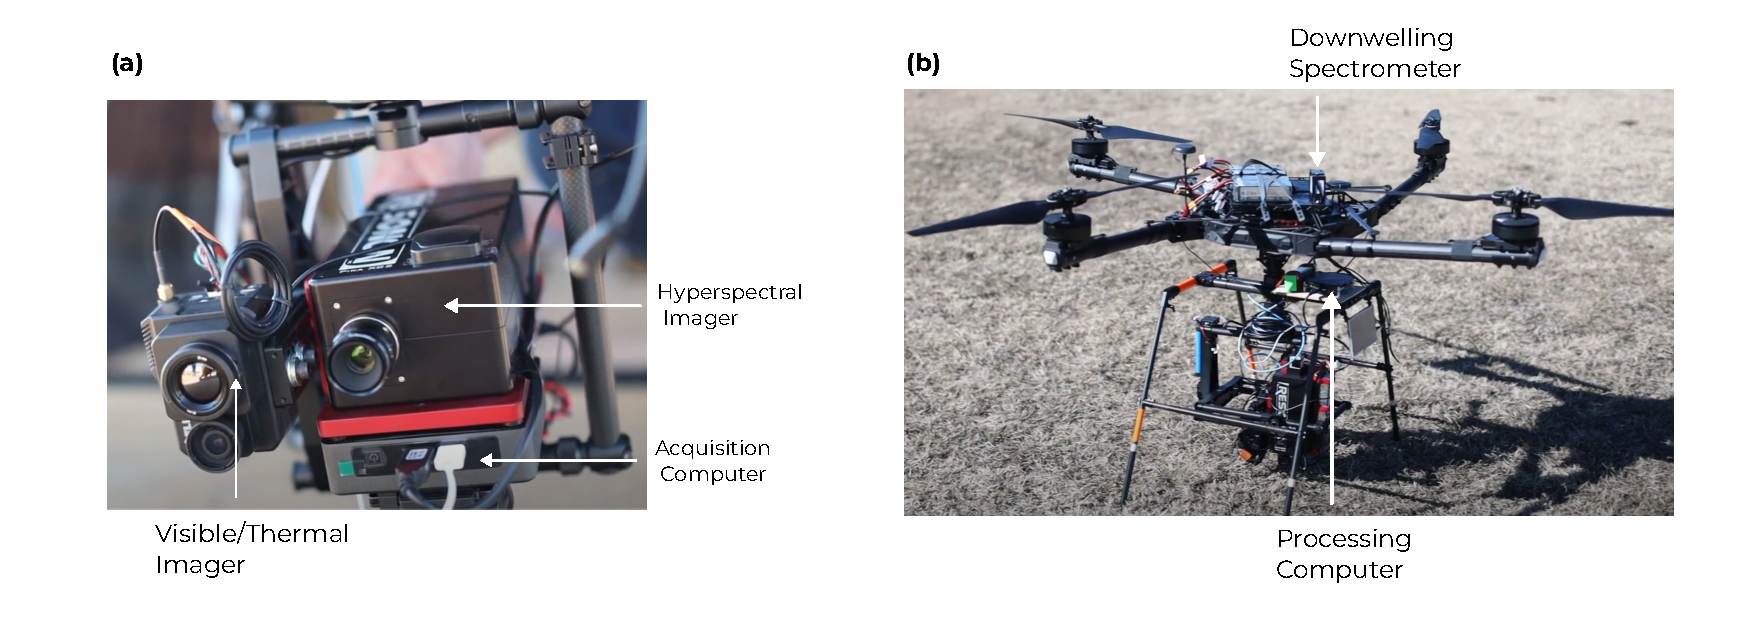
\includegraphics[width=0.85\columnwidth]{robot-team/assets/annotated-drone.pdf}
    \caption{Components of the Autonomous Drone HSI platform.}
    \label{fig:drone-components}
\end{figure}


\subsection{Real time processing of HSI imagery}

- overview of processing pipeline

\begin{figure}[h]
    \centering
    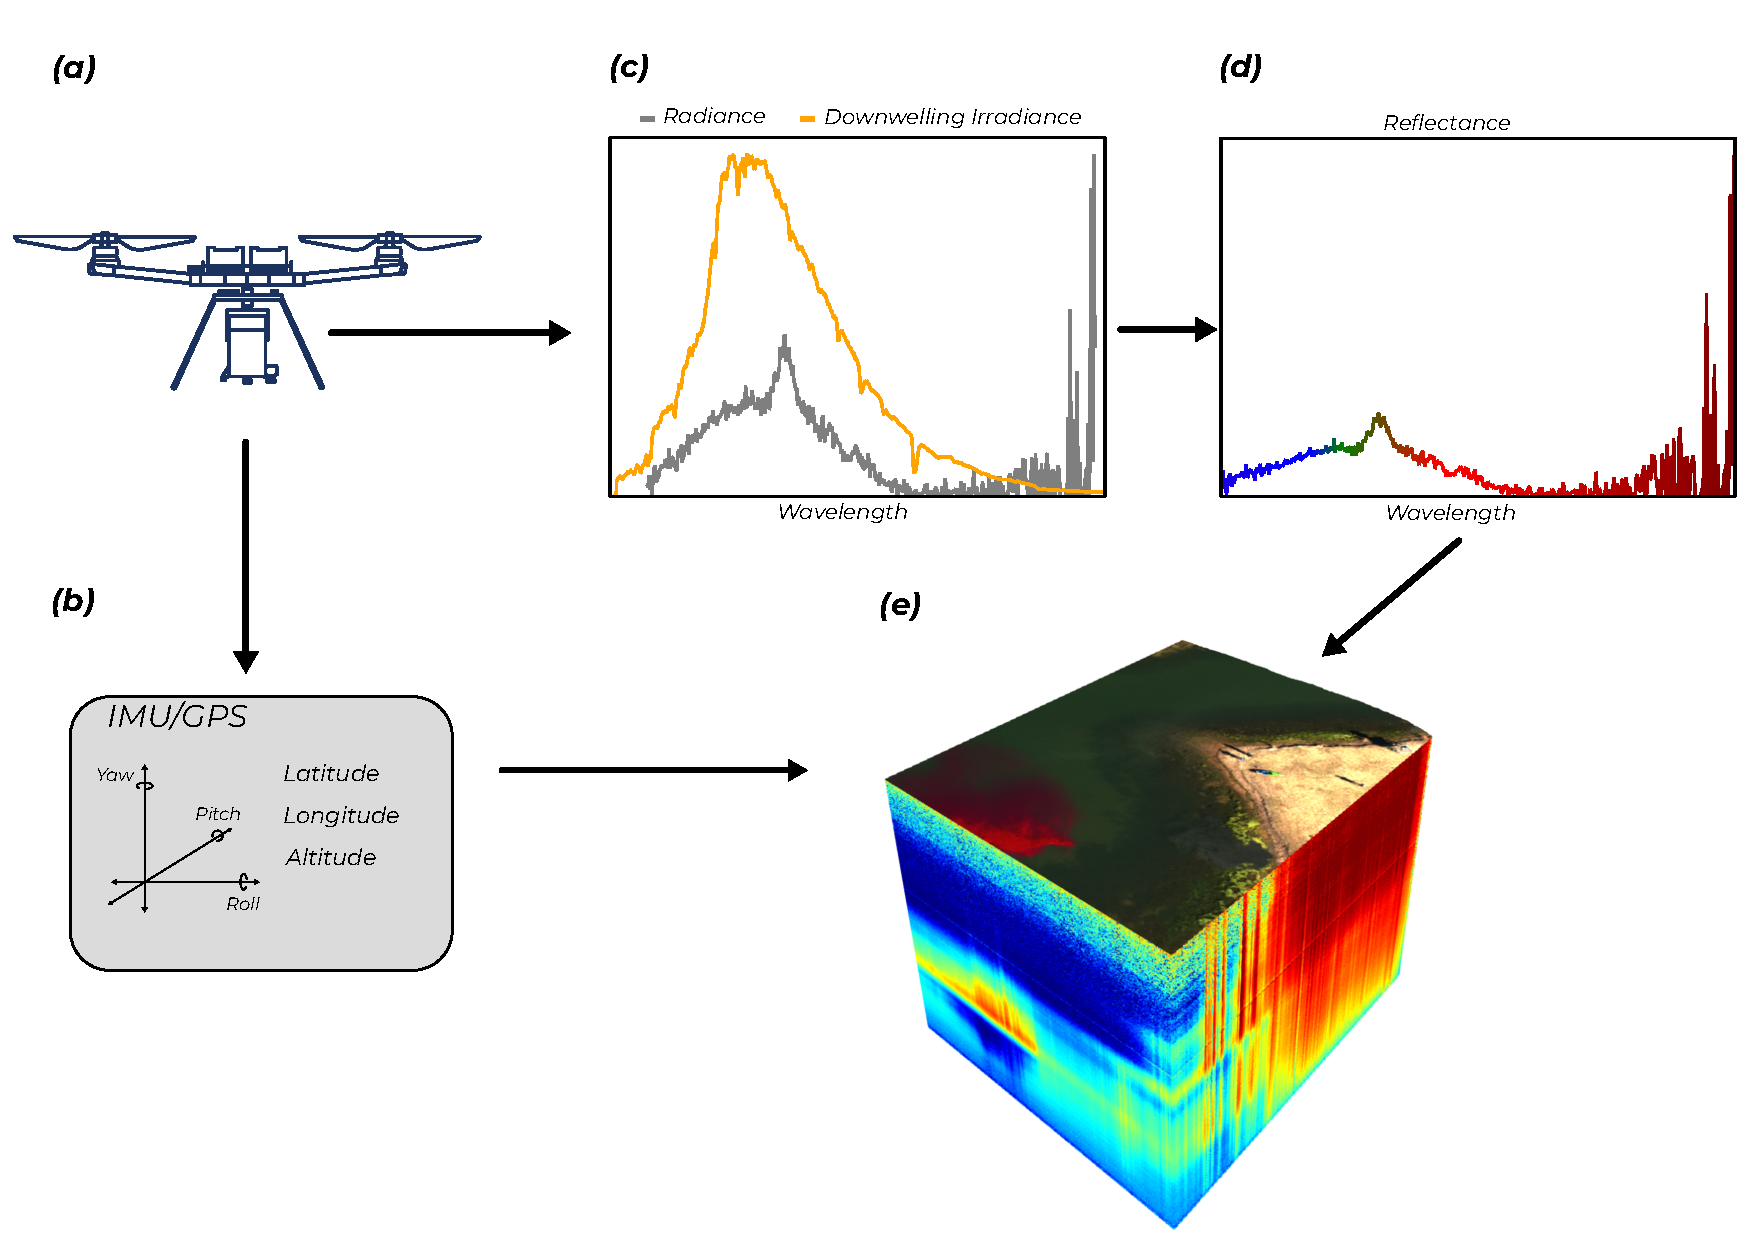
\includegraphics[width=0.85\columnwidth]{robot-team/georectification/pipeline-figure.pdf}
    \caption{Solar Irradiance spectrum captured by downwelling spectrometer.}
    \label{fig:annotated-hsi}
\end{figure}

- Collection of raw HSI by imager
- Reading stored binary (ENVI) radiance data into tensor
- Reading Flight Data 
- Interpolate flight data from IMU to match HSI times
- Reading stored downwelling irradiance spectrum 
- Interpolate irradiance spectrum to match HSI $\lambda$s 
- Conversion to Reflectance under the assumption of a Lambertian surface (perfectly diffuse)
- Georectify to obtain new coordinates
- resample to regular grid
- compute derived $\lambda$-metrics (NDVI, etc...) 
- serve result (save to HDF5 or serve via web map service over wifi) 


Georectification Procedure.
\begin{itemize}
    \item collect datacube 
    \item read HSI in ENVI format
    \item read Flight Data 
    \item interpolate flight data to HSI times 
    \item read Downwelling irradiance spectrum
    \item convert radiance to reflectance 
    \item georectify to obtain new coordinates 
    \item resample to regular grid
    \item save results to HDF5
\end{itemize}

Code and data availability via OSN and Github


\subsection{Georectification Procedure}


\begin{figure}[h]
    \centering
    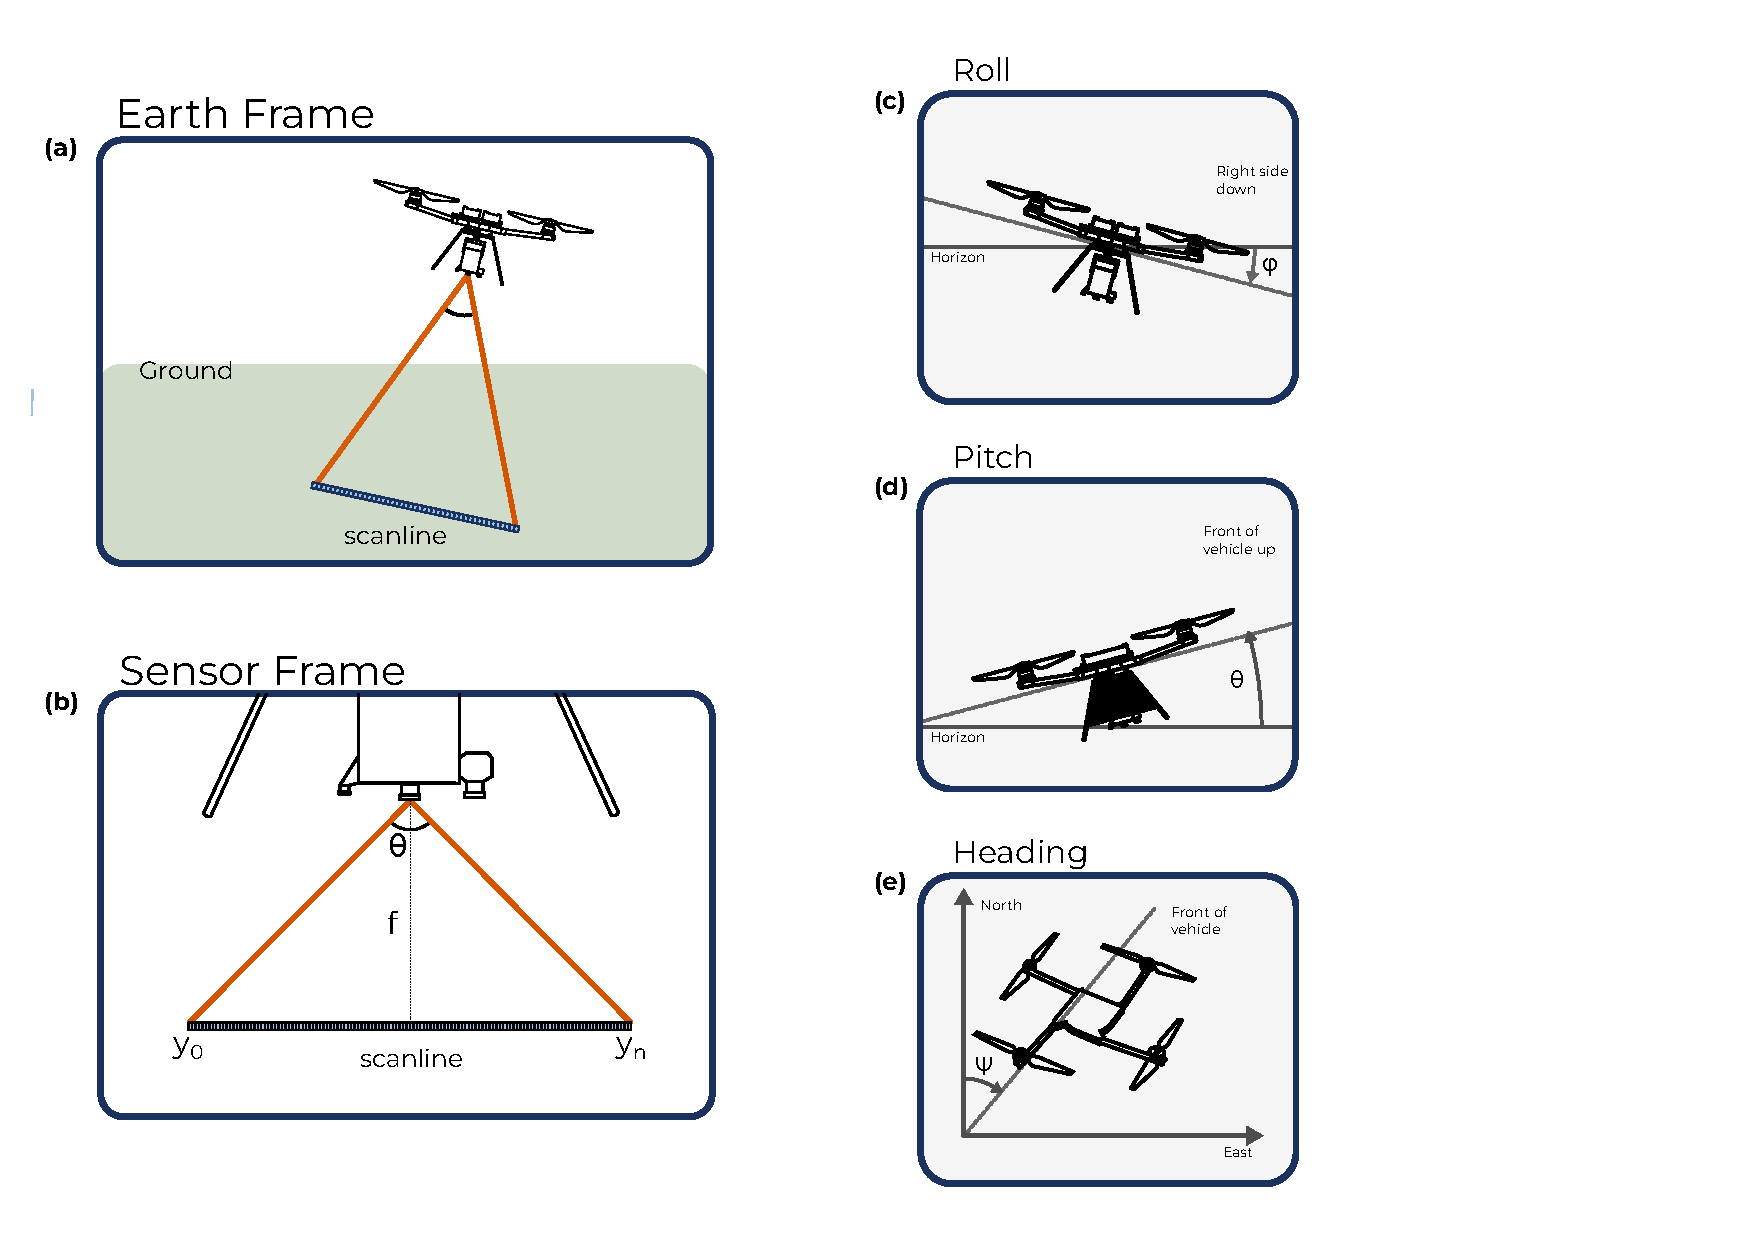
\includegraphics[width=0.85\columnwidth]{robot-team/assets/georectification.pdf}
    \caption{Visual representation of scan-line geometry for the drone based hyperspectral imaging platform.}
    \label{fig:georectification}
\end{figure}


%%%%%%%%%%%%%%%%%%%%%%%%%%%%%%%%%%%%%%%%%%
\section{Results}

\begin{figure}[h]
    \centering
    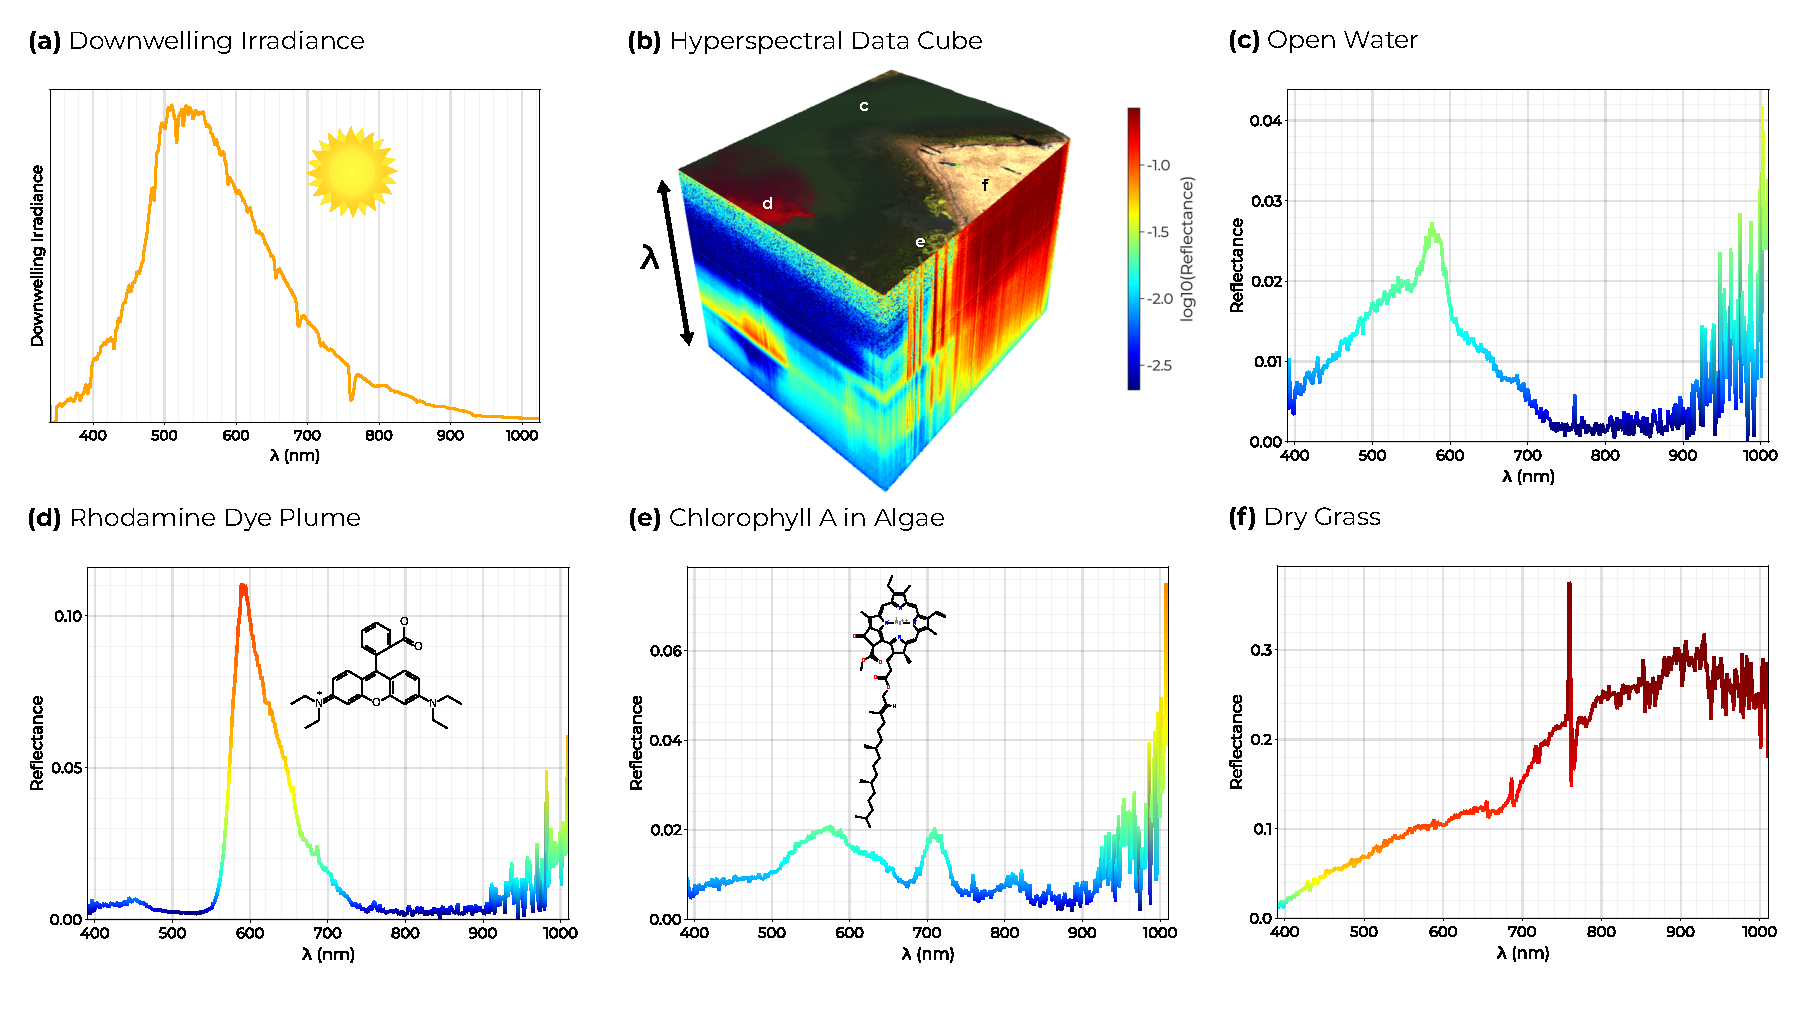
\includegraphics[width=0.85\columnwidth]{robot-team/georectification/hsi-infographic.pdf}
    \caption{Annotated view of a hyperspectral data cube showcasing sampled spectra for a variety of constituents.\label{fig:hsi-infographic}}
\end{figure}  


\begin{figure}[h]
    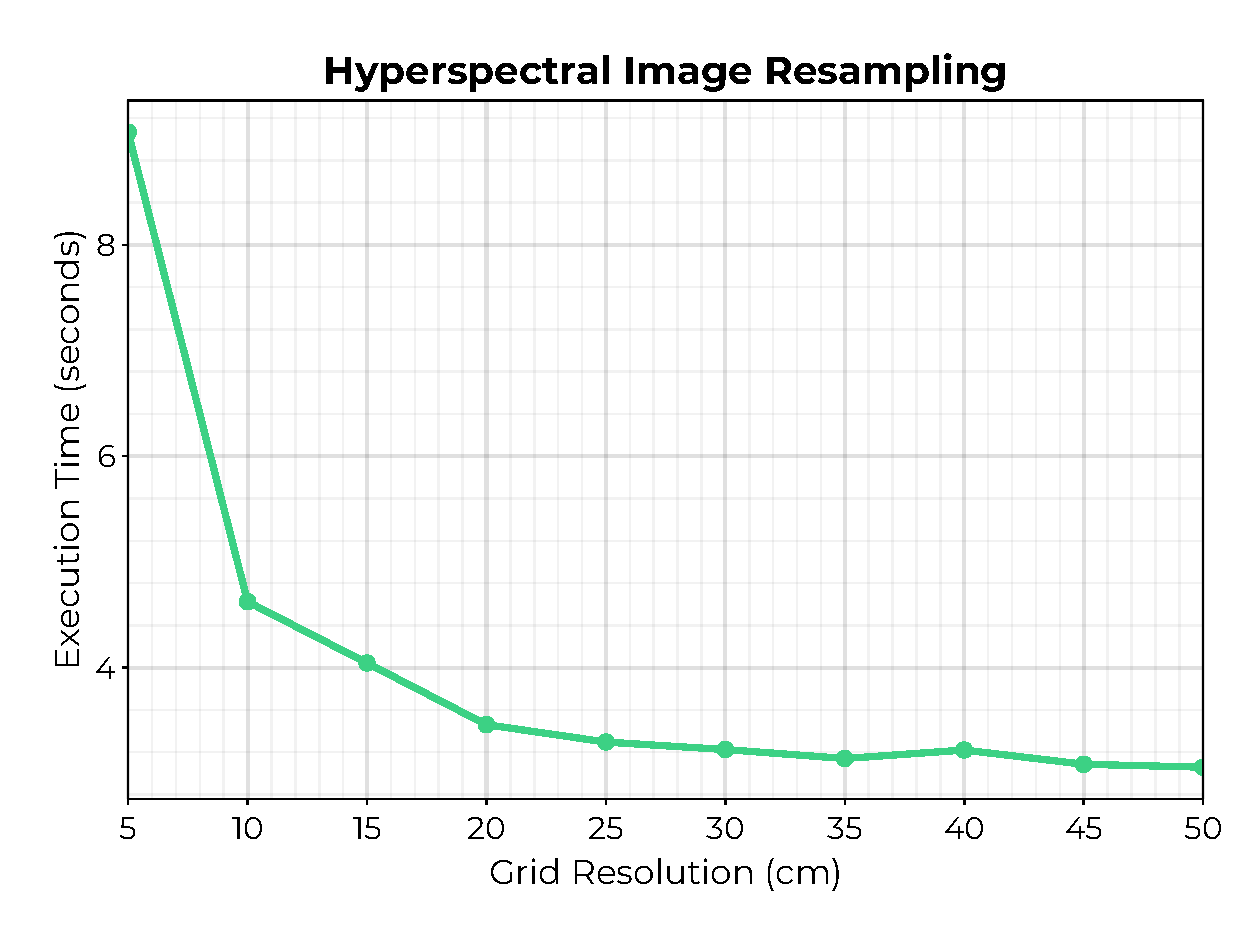
\includegraphics[width=0.85\columnwidth]{robot-team/georectification/regrid-timing.pdf}
    \caption{This is a figure. Schemes follow the same formatting. If there are multiple panels, they should be listed as: (\textbf{a}) Description of what is contained in the first panel. (\textbf{b}) Description of what is contained in the second panel. Figures should be placed in the main text near to the first time they are cited. A caption on a single line should be centered.}
    \label{fig-regridding-timing}
\end{figure}

\begin{figure}[h]
  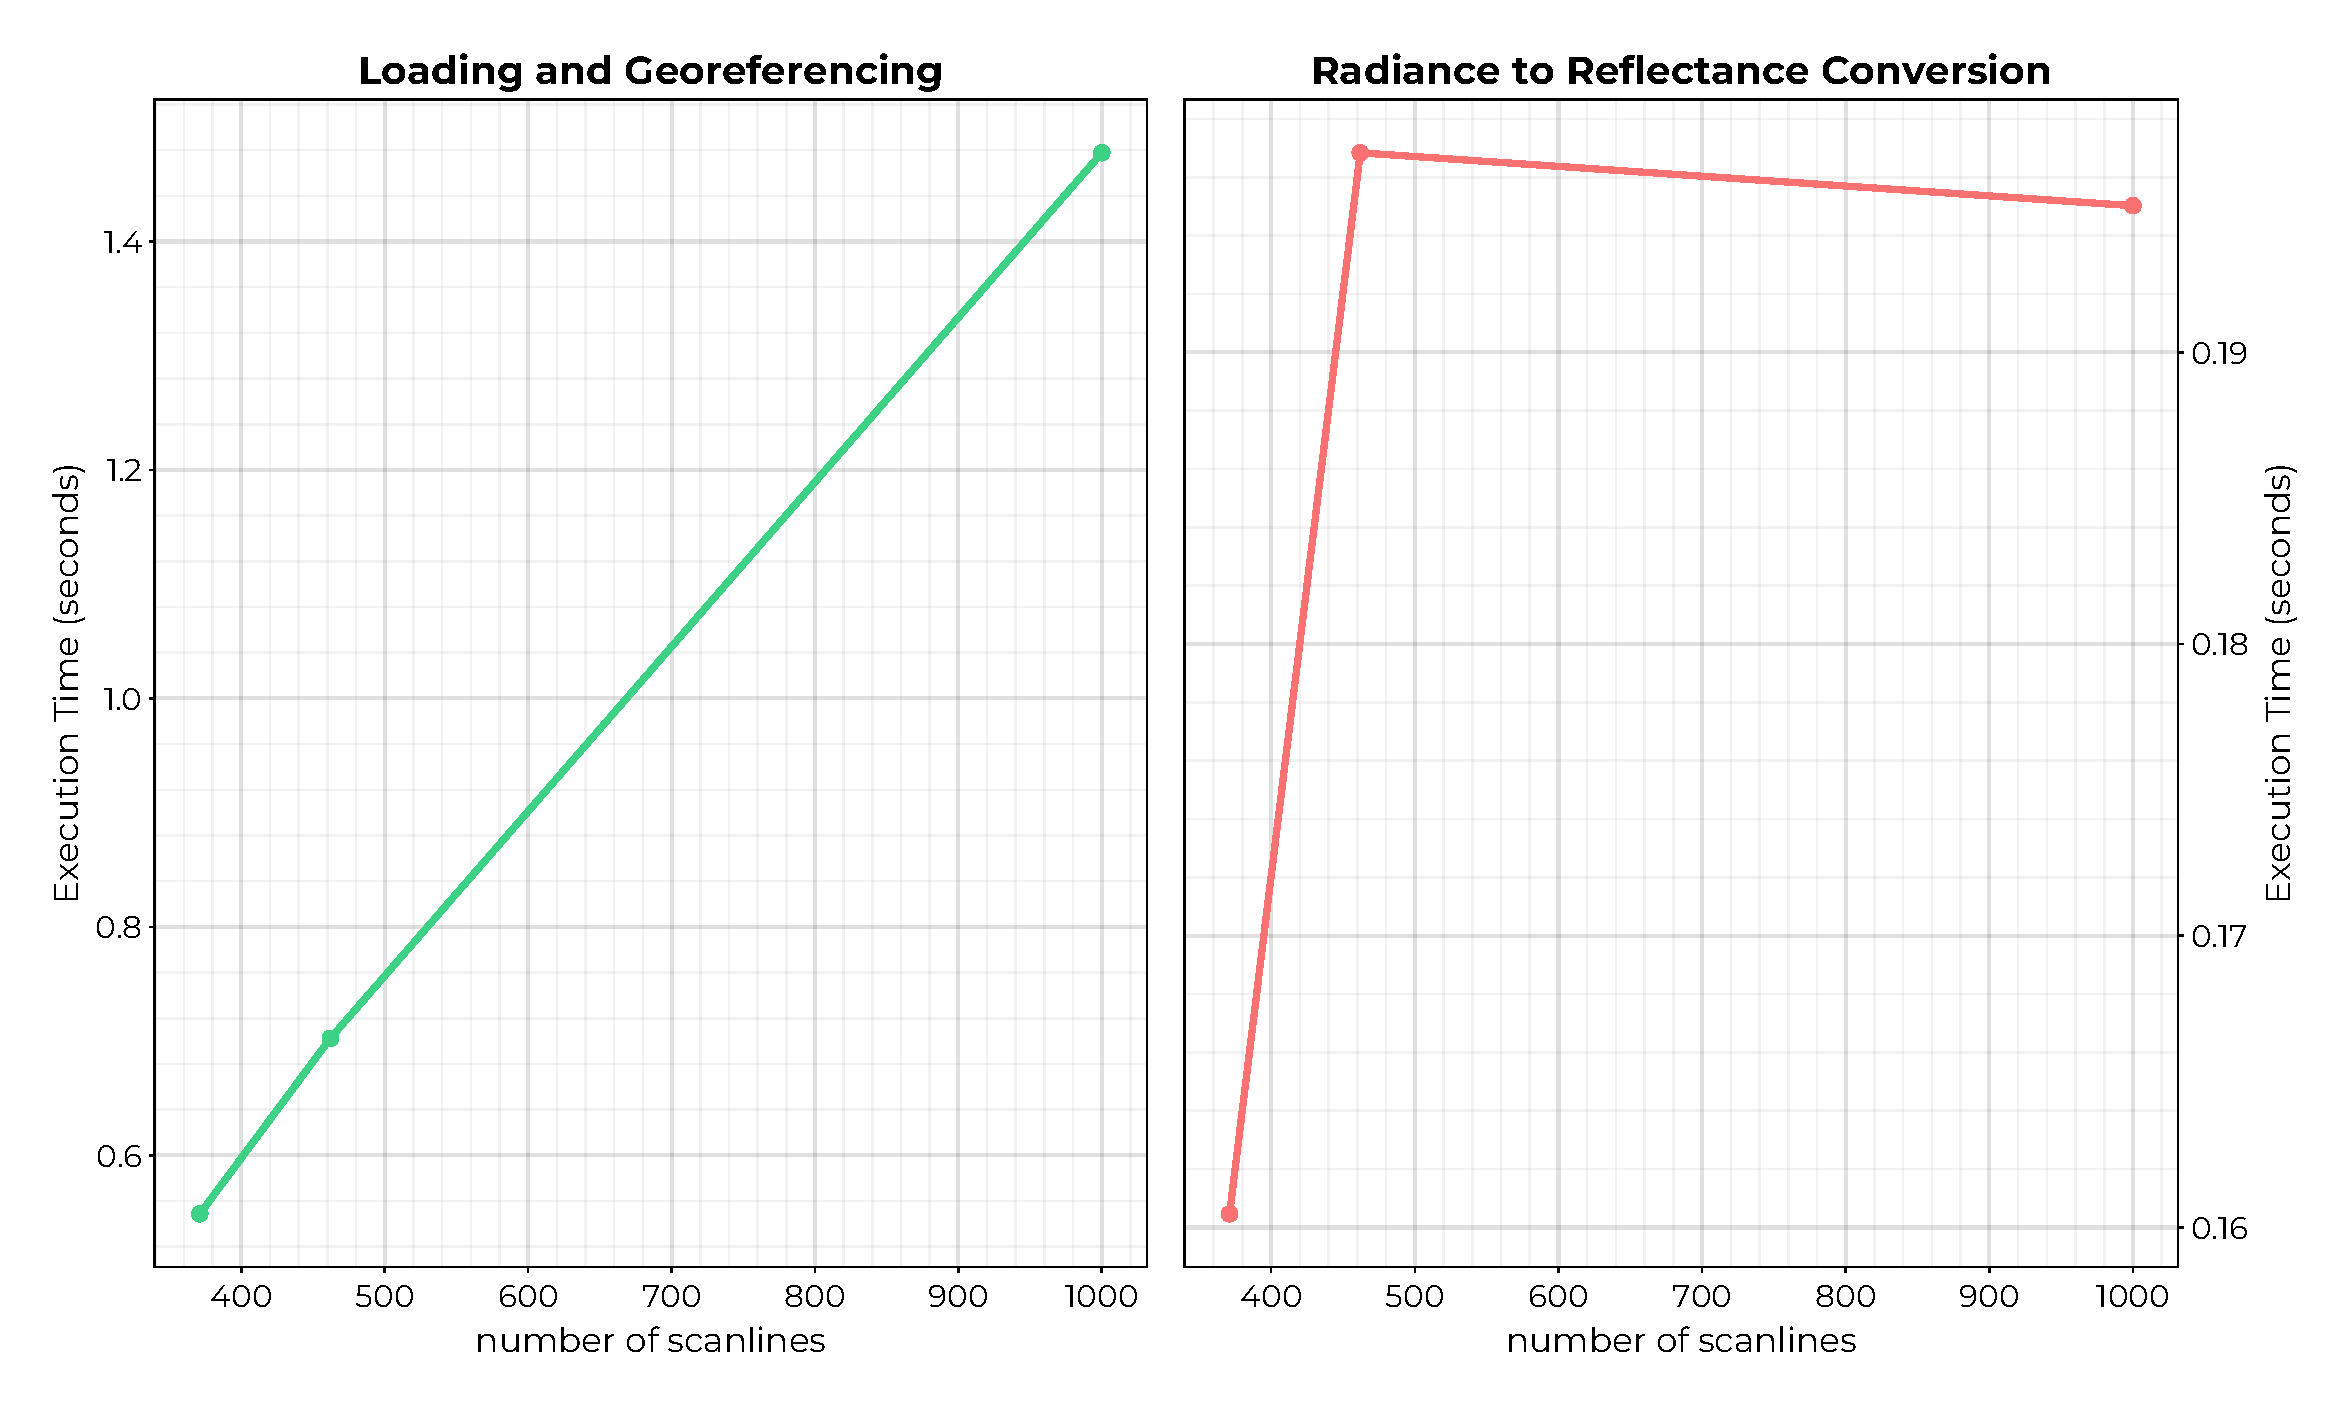
\includegraphics[width=0.95\columnwidth]{robot-team/georectification/reflectance-timing.pdf}
  \caption{Description}
  \label{fig-reflectance-timing}
\end{figure}

NOTE: we need to update these timings by first copying the HSI to the local drive (off of the external hard drive). This will probably have some effect on the read/write speeds for the test.

%% \begin{table}[h]
%% \caption{Resampling times as a function of pixel resolution.\label{tab1}}
%% \newcolumntype{C}{>{\centering\arraybackslash}X}
%% \begin{tabularx}{\textwidth}{CC}
%% \toprule
%% \textbf{Resolution (m)}	& \textbf{Execution time (s)}\\
%% \midrule
%% 0.5		&   1.434	\\
%% 0.4     &   1.545	\\
%% 0.3     &   1.673   \\
%% 0.2     &   1.802   \\
%% 0.1     &   4.026   \\
%% 0.05    &   10.537  \\
%% \bottomrule
%% \end{tabularx}
%% \end{table}


%% \begin{table}[h]
%%   \caption{Loading and Reflectance Conversion Times.\label{tab1}}
%%   \newcolumntype{C}{>{\centering\arraybackslash}X}
%%   \begin{tabularx}{\textwidth}{CC}
%%     \toprule
%%     \textbf{Number of scan lines}	& \textbf{Execution time (s)}\\
%%     \midrule
%%     371		&   2.060	\\
%%     725     &   4.227	\\
%%     1000    &   5.901   \\
%%     \bottomrule
%%   \end{tabularx}
%% \end{table}




\textbf{NOTE} Stuff to do in this section:
\begin{itemize}
    \item  Create table with processing timings for each step on a typical HSI
    \item Create second table comparing time for full processing including resampling to a variety of scales (e.g. 5 cm, 10 cm, 25 cm) We will want a version of the processing function that does not include the uncertainties and the spectral indices
    \item create pipeline visualization showing size of each of the data products and their step in the pipeline (ending with a dataproduct like the NDVI)
    \item Create a figure showing the georeferenced image on top of the satellite background 
    \item Create another figure of the entire map with a spectral index applied to one of the dye-release datasets (to demonstrate use for real-time application like oil-spill)
    \item create a figure of a sample HSI datacube in 3-d like from the previous paper with the rgb image on the top. 
\end{itemize}



%%%%%%%%%%%%%%%%%%%%%%%%%%%%%%%%%%%%%%%%%%
\section{Discussion}

- Incorporation of drone into autonomous robotic team
- Long range wireless network (ubiquiti) for data downlink
- Incorporation of edge-ML for direct determination of chemical concentration
- Utility for navigation, waste removal, etc...

Discuss drawbacks (striping in images) 

Authors should discuss the results and how they can be interpreted from the perspective of previous studies and of the working hypotheses. The findings and their implications should be discussed in the broadest context possible. Future research directions may also be highlighted.




\section{Supervised Regression with Uncertainty Quantification}

\subsection{Hyperspectral Imaging and Remote Sensing}
paper creating new spectral index for wheat rust \cite{SpectralIndexWheat} \\ 
overview of NDVI \cite{SpectralIndexNDVI} \\ 
paper using spectral indices for desertification \cite{SpectralIndexDesertification}


\subsubsection{HSI sattelite systems}
\subsubsection{HSI drone systems}
\subsubsection{Machine Learning using HSI}
add Xiao He reference here \cite{yu2021pm2}

\subsection{In-situ Measurements / Robot Teams}
\subsubsection{Meteorology}
\subsubsection{Atmospheric Sensing}
add in reference to our AQ sensor network

\subsection{Julia Programming Language}
\subsubsection{scientific computing}
\subsubsection{differentiable programming ($\partial P$)}
\subsubsection{MLJ}
discuss general \textit{learning network} framework and utilization of
Directed Acyclic Graphs for pipeline construction

basic overview of MLJ as a Julia package \cite{MLJ1}\\ 

detailed description of \textit{learning networks} \cite{MLJ2}



\section{Materials and Methods}
\subsection{Autonomous Collection and Processing of Hyperspectral Images}

website for alta x \cite{freeflyAltaX}

\begin{equation}
  R = \pi \frac{L}{E}
\end{equation}



\subsection{Georectification}
paper by Muller \cite{muller-georeferencing} \\
paper by Baumker \cite{GeorectificationBaumker} \\
paper by Mostafa \cite{GeorectificationMostafa} \\



NOTE: need to double check \cite{muller-georeferencing} for convention used ($\Phi$ vs $\phi$)

Heading correction due to longitude deviation in UTM system:
\begin{equation}
  \kappa_{\text{geodetic}} = \kappa_{\text{geographic}}-\tan^{-1}\left( \sin\Phi \tan(\lambda-\lambda_{cm}) \right)
\end{equation}

scale factor:
\begin{equation}
  s = \frac{z_{\text{sensor}}-z_{\text{ground}}}{f}
\end{equation}

\begin{equation}
  \begin{pmatrix}
    x \\ y \\ z
  \end{pmatrix}_{\text{Object}}^{\text{UTM}} =
  f_{\text{geo}}^{\text{UTM}}\begin{pmatrix}
    \lambda \\
    \Phi \\
    z
  \end{pmatrix}_{\text{GPS}}^{\text{geo}} + sT_{\text{IMU}}^{\text{UTM}}R_{\text{sensor}}^{\text{IMU}}(\kappa, \phi, \omega)\begin{pmatrix}
    0 \\
    y_i \\
    f
  \end{pmatrix}_{\text{object}}^{\text{sensor}}
\end{equation}




\subsection{In-situ Data Collection via Robotic Sentinels}

autonomous boat website \cite{Otter}


\subsubsection{data collection process}
\subsubsection{Data Collocation}

\subsubsection{CO}
\subsubsection{CDOM}
\subsubsection{HDO}
\subsubsection{$Na^{+}$}
\subsubsection{$Ca^{2+}$}
\subsubsection{Other Targets}

\subsubsection{Feature Engineering with Remote Sensing Indices}
include discussion of PCA as well as Standardization


\subsection{Exploratory Data Analysis}
\subsubsection{Variable Correlations}

\begin{figure}[h]
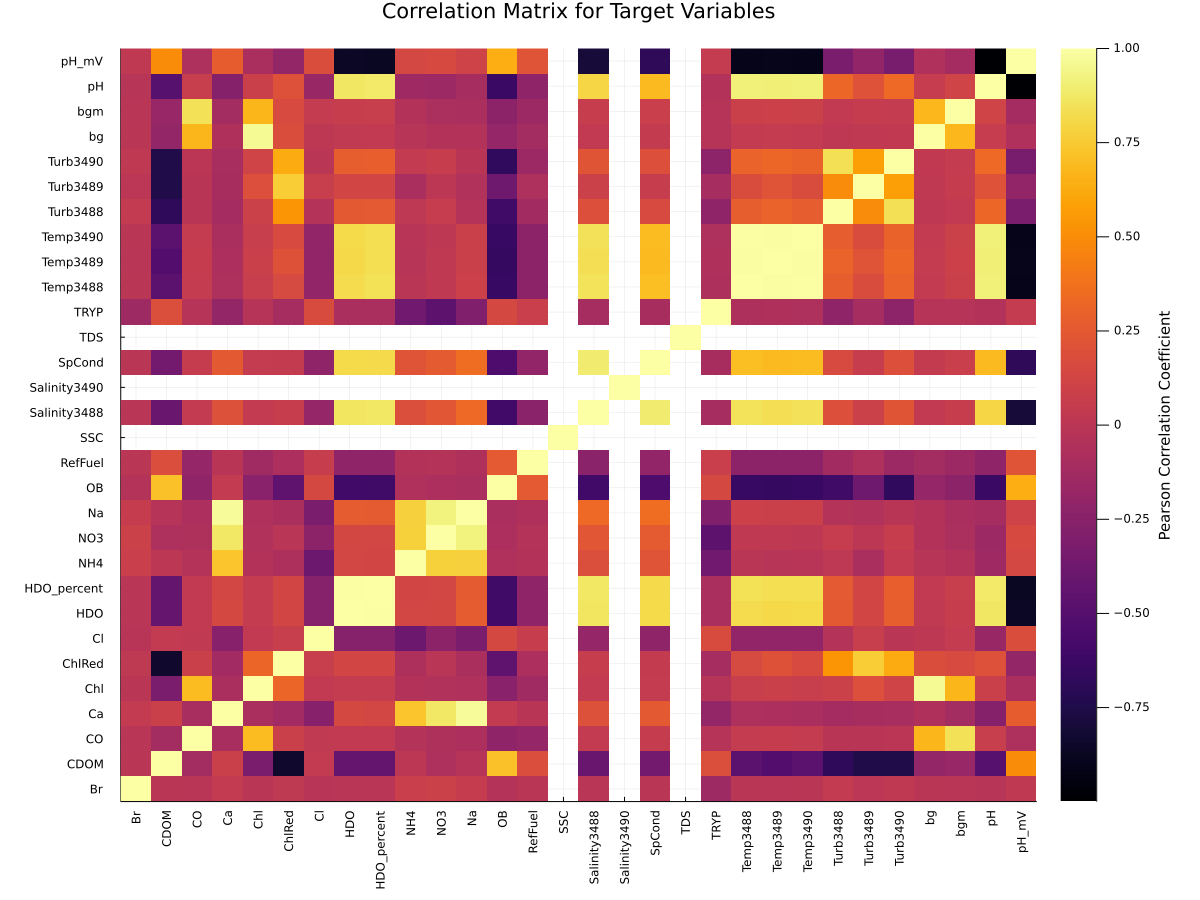
\includegraphics[width=0.85\columnwidth]{robot-team/supervised-2/correlation/target_cor.png}
\caption{Correlation Matrix for Target variables measured by the boat.\label{target_cor}}
\end{figure}

\begin{figure}[h]
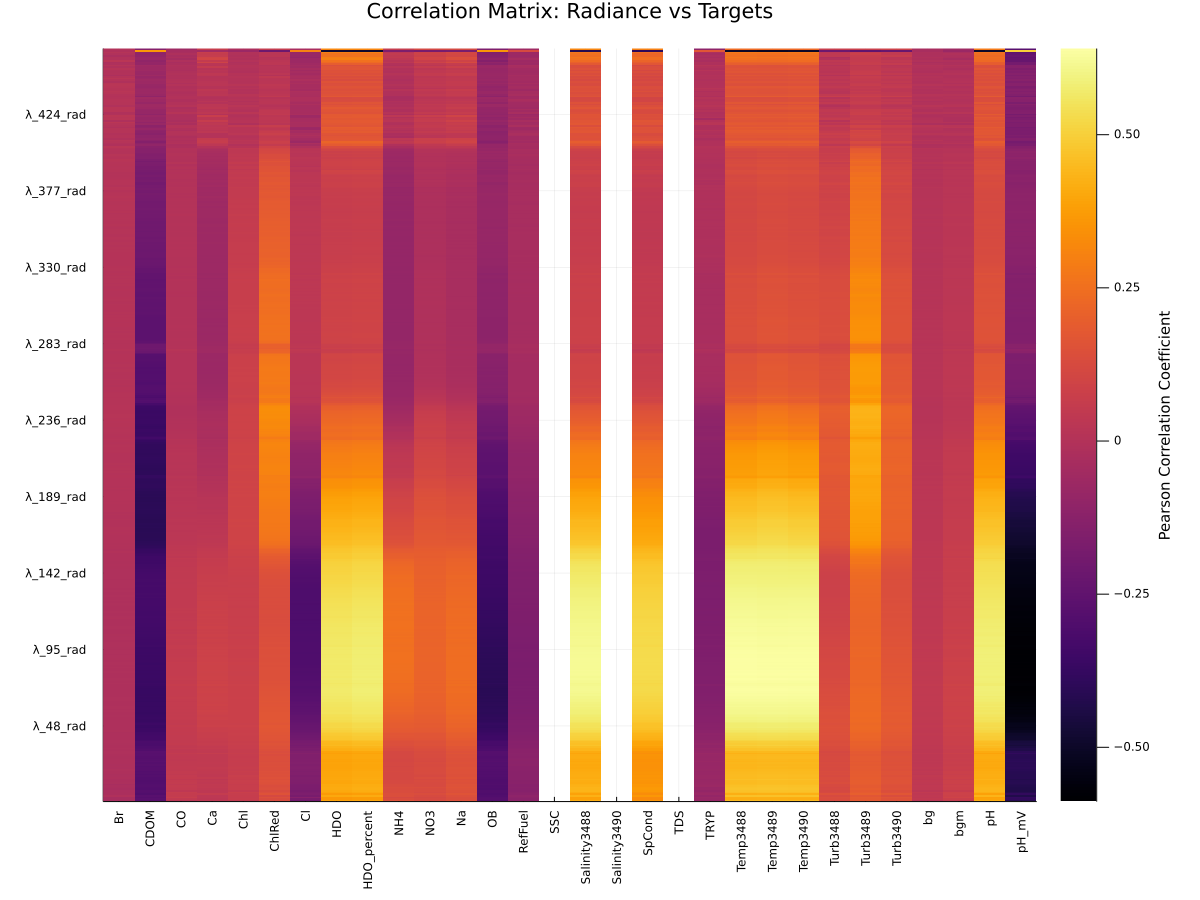
\includegraphics[width=0.85\columnwidth]{robot-team/supervised-2/correlation/radiance_cor.png}
\caption{Correlation Matrix for Radiance measurements versus Target Variables.\label{rad_cor}}
\end{figure}

\begin{figure}[h]
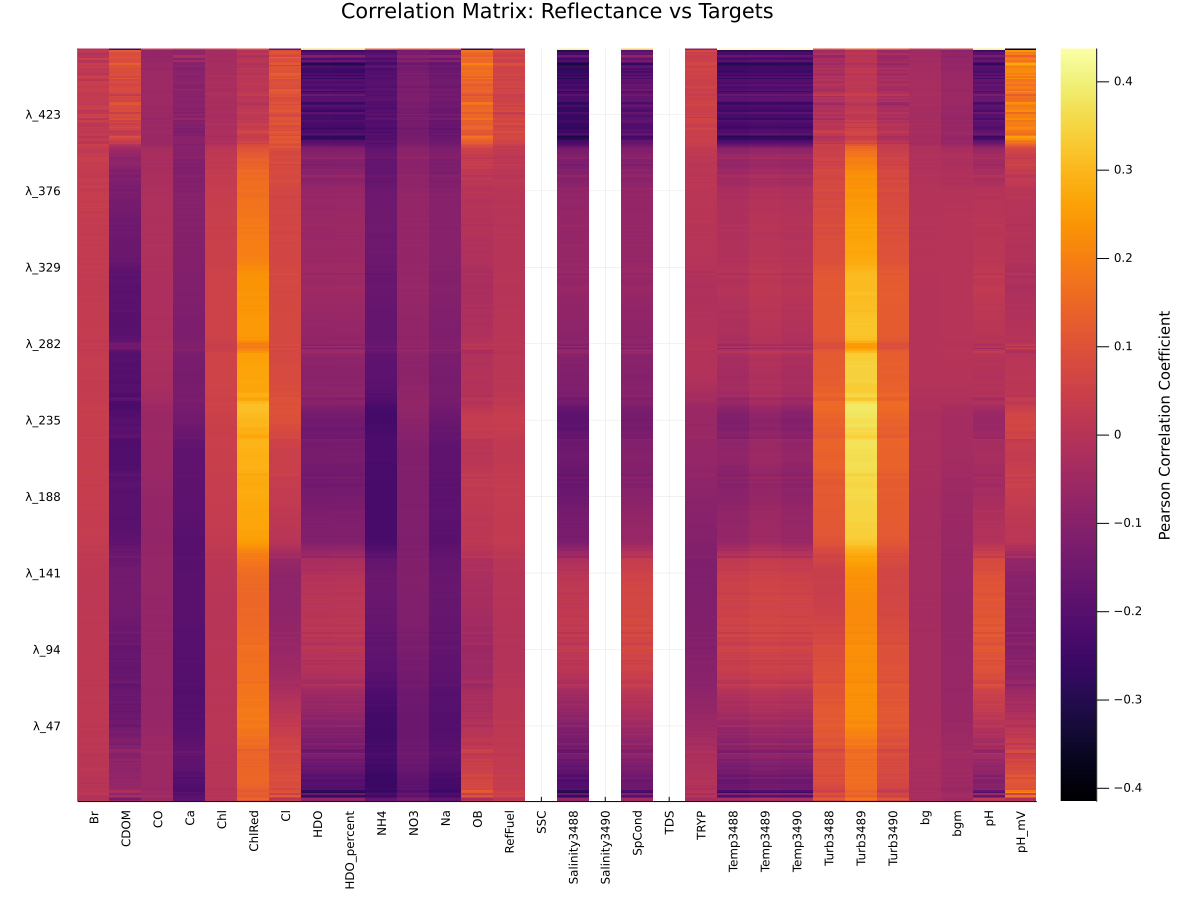
\includegraphics[width=0.85\columnwidth]{robot-team/supervised-2/correlation/reflectance_cor.png}
\caption{Correlation Matrix for Reflectance measurements versus Target Variables.\label{ref_cor}}
\end{figure}

\begin{figure}[h]
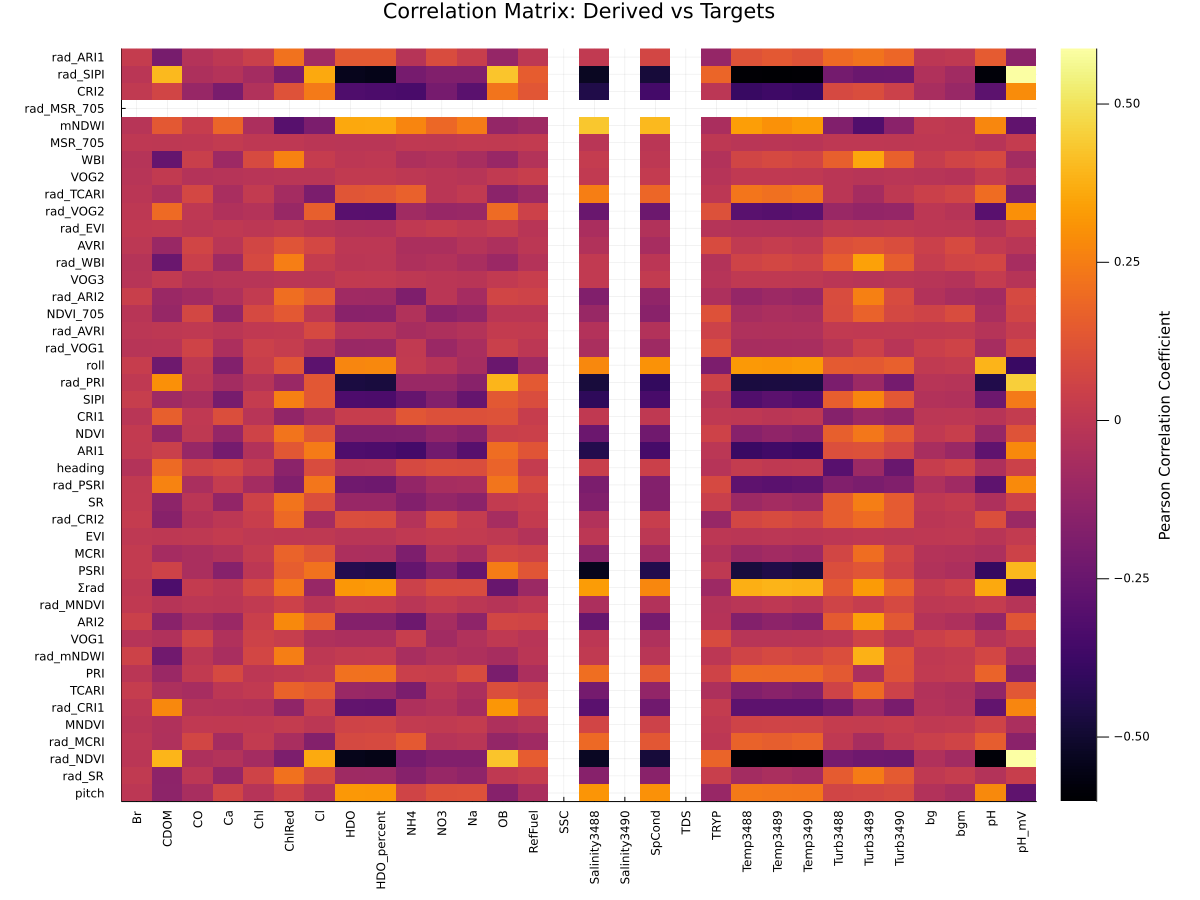
\includegraphics[width=0.85\columnwidth]{robot-team/supervised-2/correlation/derived_cor.png}
\caption{Correlation Matrix for derived measurements versus Target Variables.\label{derived_cor}}
\end{figure}



\subsubsection{Machine Learning Models}
include Linear Models, Neural Networks, Decision Trees, Bagging, Boosting, and Stacking\\

The field of Machine Learning has seen the invention of a plethora of models able to perform inference for regression tasks. Naturally, this leads to the challenge of evaluating which model is best for a given problem. In 1992 David Wolpert developed the notion of Stacked Generalization to divorce arbitrary human choice from the model selection process. [1] The key idea is as follows: fit an instance of each model compatible with your dataset. Each model learns different features of the data so that an adjudicating model (called the super-learner) can then be trained to map the predictions from each individual learner to a final output prediction. This is incredibly easy to accomplish in the Julia programming language via the MLJ machine learning framework [2]. We train a variety of learners including artificial neural networks, bagged decision trees, boosted decision trees, polynomial regressors, quantile regressors, LASSO regressors, and K-nearest-neighbors regressors. To ensure proper data hygiene, individual learners are first trained on separate cross validation folds so as not to bias the super-learner. After training the super-learner, each individual model is then trained on the full dataset to produce the best possible model.


paper on stacking \cite{ModelStacking}

\subsection{Model Analysis}
aleatoric and epistemic uncertainty

The black-box nature most machine learning methods makes it difficult to consider how errors propagate through a trained model during the inference process. For many problems such as image classification this is not an issue, however, in physical sensing error considerations are vital to establish detection limits and prediction confidence. Typically, there are three considerations we must make: measurement uncertainty– how much we can trust our model’s inputs, measurement representativeness– how well each data point represents data within a local neighborhood, and model error– how far the prediction is from the true value. Machine learning models are typically trained to minimize the model error. The Julia programming language makes it possible to handle all three. 


To address measurement uncertainty, we take advantage of Julia’s advanced automatic differentiation capabilities to enable differentiable programming (∂P). This means that we can take derivatives of our trained ML model with respect to each input feature to perform a sensitivity analysis. The final output uncertainty is then given via linear error propagation theory. [5]

Measurement representativeness can be trickier to handle. For example, in fluids it is common for two species to form a mixing layer that presents as a sharp discontinuity in measurement values. To quantify the degree to which neighboring points diverge we compute the average deviation across input measurements in a neighborhood around each data sample. This information can then be presented with model outputs to identify the regions where our model is valid. Similarly for ensemble ML models we compute the prediction deviation across all base learners to identify the representativeness of a data sample. Inputs that cause a large spread in base learner predictions indicate low representativeness in the training set. This analysis can then be used to plan further data collection missions that minimize time spent collecting data we have already present in our models. 

\subsubsection{Uncertainty Propagation via ($\partial P$)}

\subsubsection{Feature Ranking via SHAP values}

shape value paper used in ShapML.jl \cite{SHAPvalues1}

\subsubsection{Data Representativeness}
i.e. the average deviation across pixels used average during collocation process.
Also, we can look at relative disagreement between model predictions in bagged ensemble. 

\section{Results}
\subsection{CO}

\begin{figure}[h]
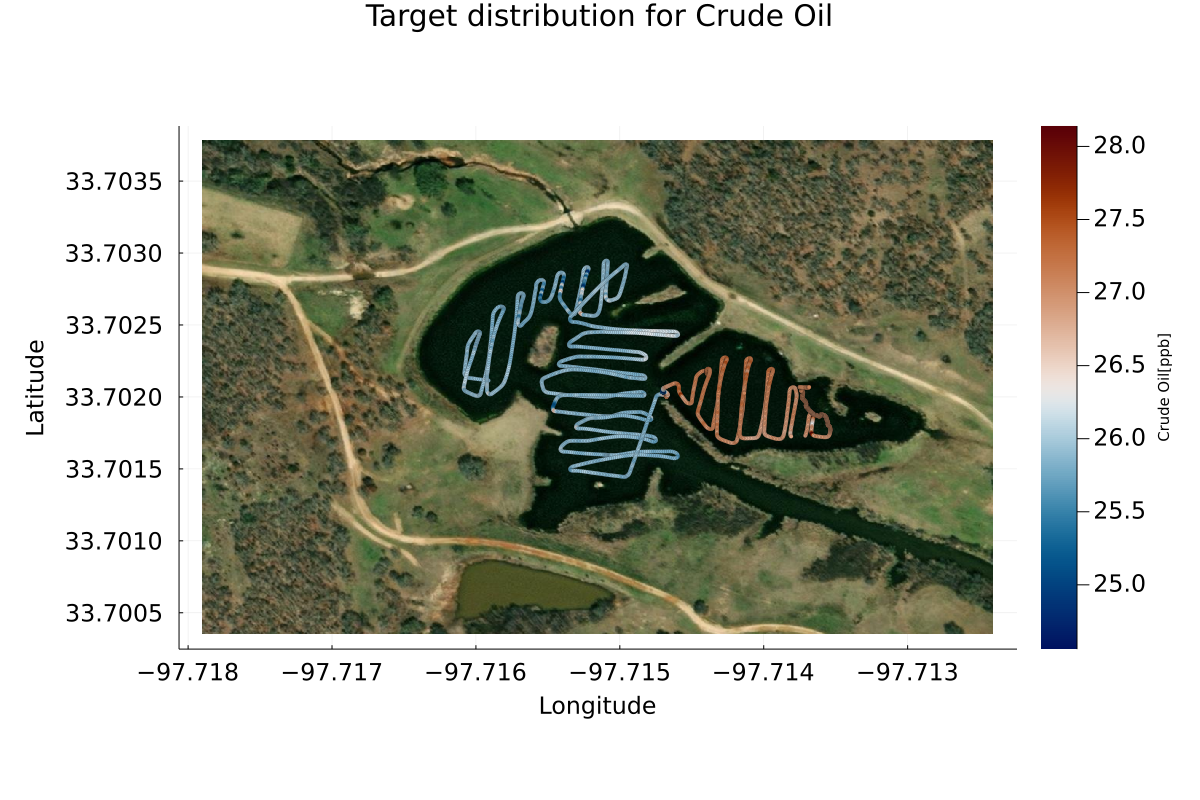
\includegraphics[width=0.85\columnwidth]{robot-team/supervised-2/CO/CO_dataMap.png}
\caption{Target distribution of CO at Scotty's Ranch.\label{CO_targetMap}}
\end{figure}

\begin{figure}[h]
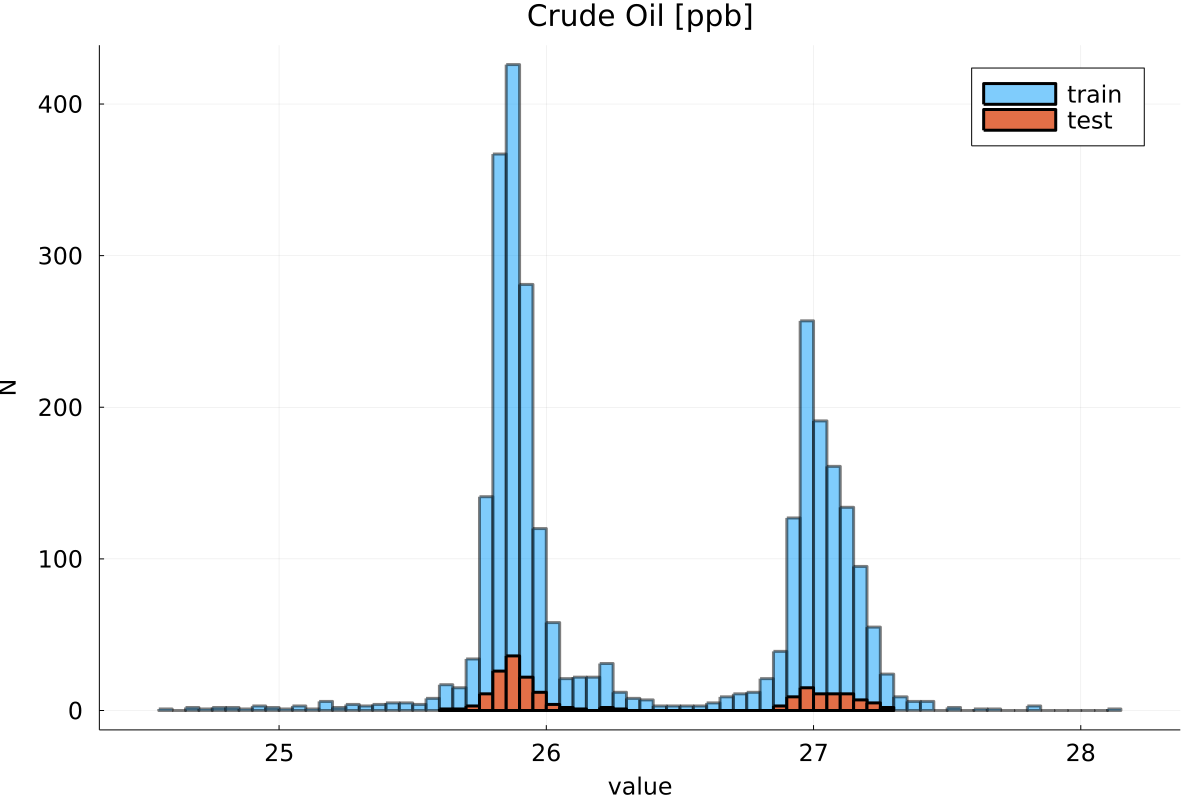
\includegraphics[width=0.85\columnwidth]{robot-team/supervised-2/CO/CO_train-test_hist.png}
\caption{Stratified train-test split for CO.\label{CO_trainTestHist}}
\end{figure}

\begin{figure}[h]
  \begin{subfigure}{0.5\textwidth}
    \centering
    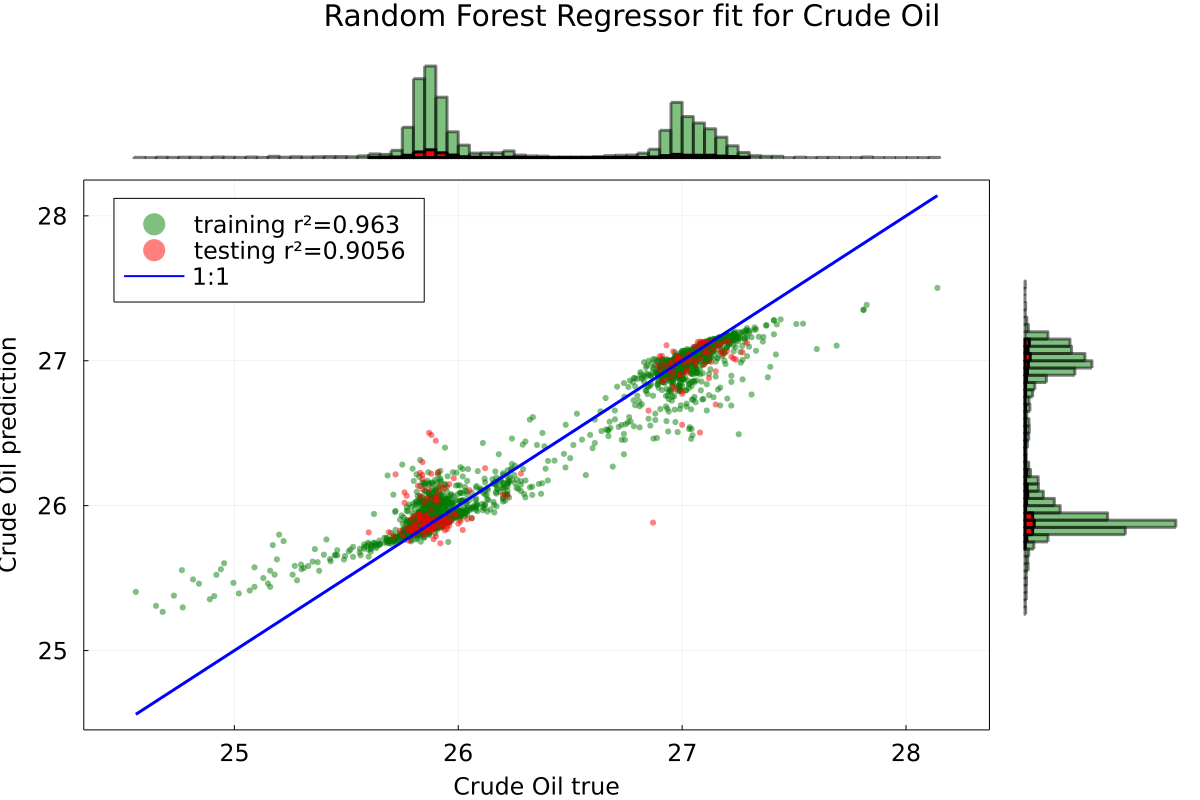
\includegraphics[width=0.95\linewidth]{robot-team/supervised-2/CO/rfr_CO_scatter.png}
  \end{subfigure}
  \begin{subfigure}{0.5\textwidth}
    \centering
    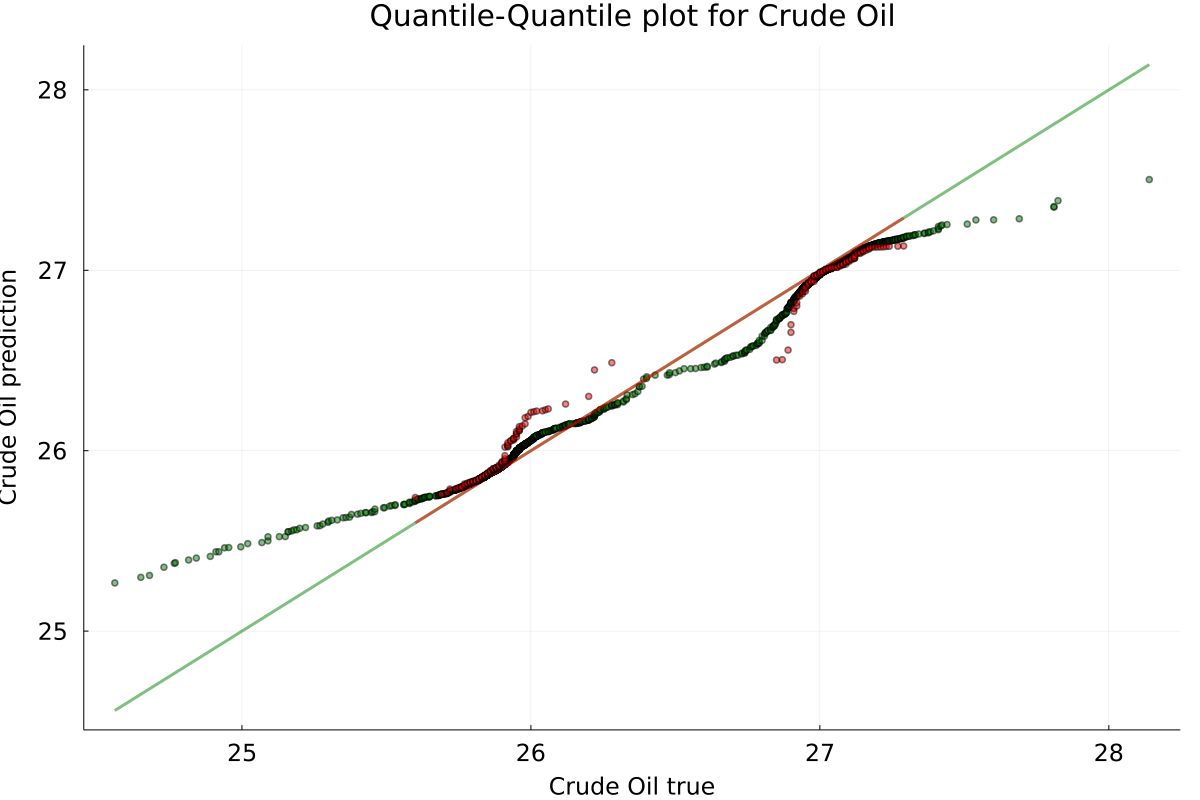
\includegraphics[width=0.95\linewidth]{robot-team/supervised-2/CO/rfr_CO_qq.png}
  \end{subfigure}
  \caption{(\textbf{a}) Scatterplot for the trained random forest Crudo Oil model. (\textbf{b}) Quantile-Quantile plot for the same fit.}
  \label{CO_fitresult}
\end{figure}



\begin{figure}[h]
    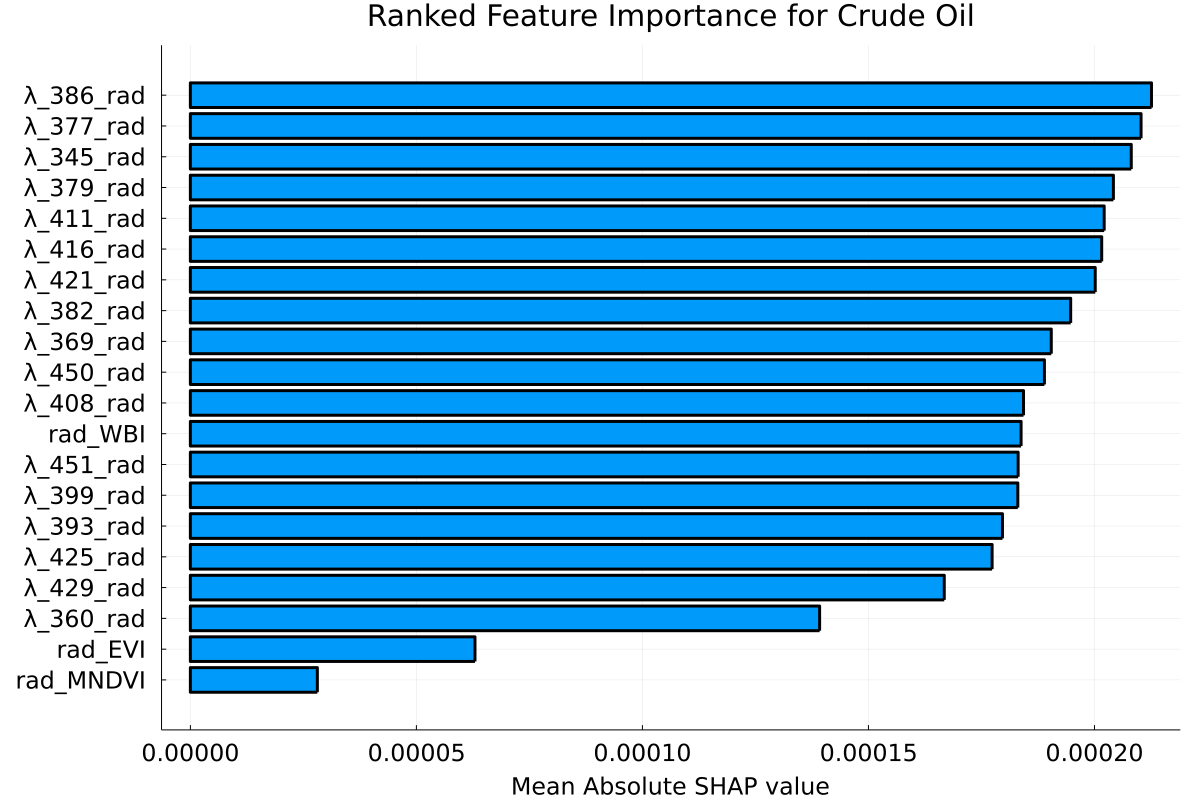
\includegraphics[width=0.85\columnwidth]{robot-team/supervised-2/CO/rfr_CO_featureImportance.png}
    \caption{Ranked feature importance for Crude Oil. Importance is determined via mean absolute SHAP value. \label{CO_shapely}}
\end{figure}






\section{Methods for Unsupervised Classification of Hyperspectral Scenes in Novel Environments}

\subsubsection{Unsupervised Classification}
\begin{figure}[h]
  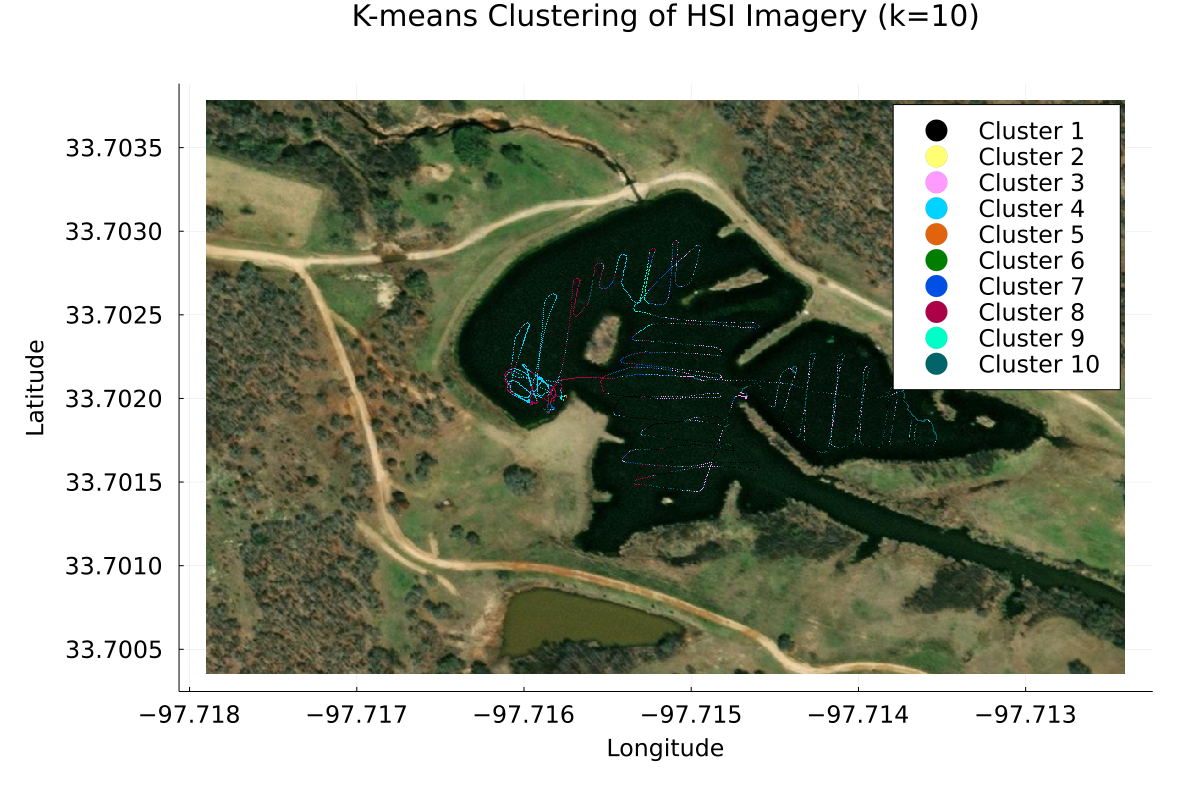
\includegraphics[width=0.85\columnwidth]{robot-team/unsupervised/clustering.png}
  \caption{Unsupervised clustering of hyper-spectral image data using the K-means algorithm.\label{clustering}}
\end{figure}



